\scanpage{48}
\deleted{tés, les morphismes \uline{toutes} les correspondances \inserted{co}homologiques (en vert\unsure{u}
du thorème de Thom rappelé plus haut). On trouve donc un foncteur
pleineme\deleted{t}nt fidèle de cette catégorie dans celle d es vectoriels
gradués \deleted{\unsure{de d}} positivement de dim. finie sur $\underline{F}_2$ , qui est déjà abélien%
ne, et si on veut rendre comme plus haut $\underline{F}_2(-1)$ inversible, on trouve
tous les vectoriels gradués de dim. finie sur $\underline{F}_2$ . C'est un peu trop
trivial comme structure, et on peut faire mieux, \deleted{en prenant comme}}

\inserted{Pour trouver une catégorie universelle,}
\deleted{\unsure{correspondances. Pour ceci}} on associe à toute X \deleted{\unsure{le sous-anneauensemble}}
\deleted{\unsure{de}} l'ensemble \inserted{S(X)} des sous-variétés \deleted{S(X)} de X, modulo équivalence homolo%
gique. Donc S(X) \handwritten{$\subset$} $H^{\cdot}(X)$, et on prouve qu'on trouve en fait un sous-
anneau de $H^{\cdot}(X)$ (grâce à un théorème de Thom qui caractérise S(X) en
termes d'opérations de Steenrod, cf plus bas). On prouve de même
(par le même théorème) que les S(XxY) sont stables par composition des
correspondances cohomologiques\deleted{\illegible{1}}( cela ne semble pas trivial, puisque
les S(X) ne sont pas stables par Gysin...). D'o\unsure{û|ù} une catégorie addi-
tive dont les objets sont ceux de C, les flêches sont les S(XxY),
Il semble qu'elle doive jouer le rôle universel que j'ai envisagé
plus haut. En tous cas, sa définition géo\deleted{é}m\deleted{m}étrique est fort simple !
Nous allons en donner une interpétation algébrique. P\u{o}ur ce\deleted{i}c\deleted{c}i,
considérons l'anneau des opérations cohomologiques \inserted{``stables''} \deleted{\deleted{additives sur} i.e.}
\margin{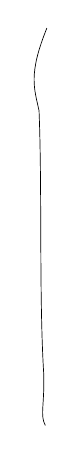
\begin{tikzpicture}[x=0.01cm,y=0.01cm]\draw[line width=.25pt] (17,505) .. controls (-7,446) and (1,428) .. (7,400) .. controls (11,300) and (7,160) .. (13,65) .. controls (14,25) and (8,13) .. (15,0);\end{tikzpicture}}
\deleted{\inserted{des endomorphismes du}}
\margin{\handwritten{\unsure{Faux !|?}}}
\deleted{\deleted{le} foncteur X \quad $H^{\cdot}$(X) qui sont additifs, et qui en degré zéro se
réduisent à un multiple de l'identité.} C'est un anneau gradué, avec
application diagonale anticommutative, \inserted{i.e. commutative (car. 2 !)} associative et unitaire. Son
dual gradué est une algèbre \inserted{graduée an\unsure{ti|tt}commutative donc \deleted{commutative},} commutative,avec application diagonale
associative et unitaire; il est réduit à $\underline{F}_2$ en degré zéro. Donc il
corespond à un schéma en groupes \handwritten{aff}ine G sur $\underline{F}_2$ , qui est d'ailleurs
le foncteur des $\otimes$-automorphismes \inserted{additifs} du foncteur $H^{\cdot}$ sur C \inserted{\handwritten{qui opèrent
trivialement sur \deleted{\unsure{l'objet}} $H^{\unsure{1}}(S^1)$. \deleted{\illegible{1}}}}

\margin{\handwritten{47}}
